\documentclass[12pt,a4paper]{article}
\usepackage[utf8]{inputenc}
\usepackage[T1]{fontenc}
\usepackage[spanish]{babel}
\usepackage{amsmath}
\usepackage{amsfonts}
\usepackage{amssymb}
\usepackage{graphicx}
\usepackage[width=18.00cm, height=26.00cm]{geometry}
\author{Gabriel Octavio Lozano Pinzón}
\title{Laboratorio 9}

\begin{document}
\maketitle
Para este laboratorio se usa el notebook especificado para buscar el mejor asset para invertir a 6 meses y a 2 años. En el caso de 6 meses el asset es FTSV, el desempeño del algoritmo se puede ver en la Figura \ref{fig:inversion6meses} y el comportamiento de acuerdo a yahoo finance se puede ver en la Figura \ref{fig:yahoo6meses}.  \\

Para el caso de los dos años la acción que se usa es AXSM cuyo resultado del algoritmo está en la Figura \ref{fig:inversion2anos} y el resultado por yahoo finance se muestra en la Figura \ref{fig:yahoo2anos}.



\begin{figure}
	\centering
	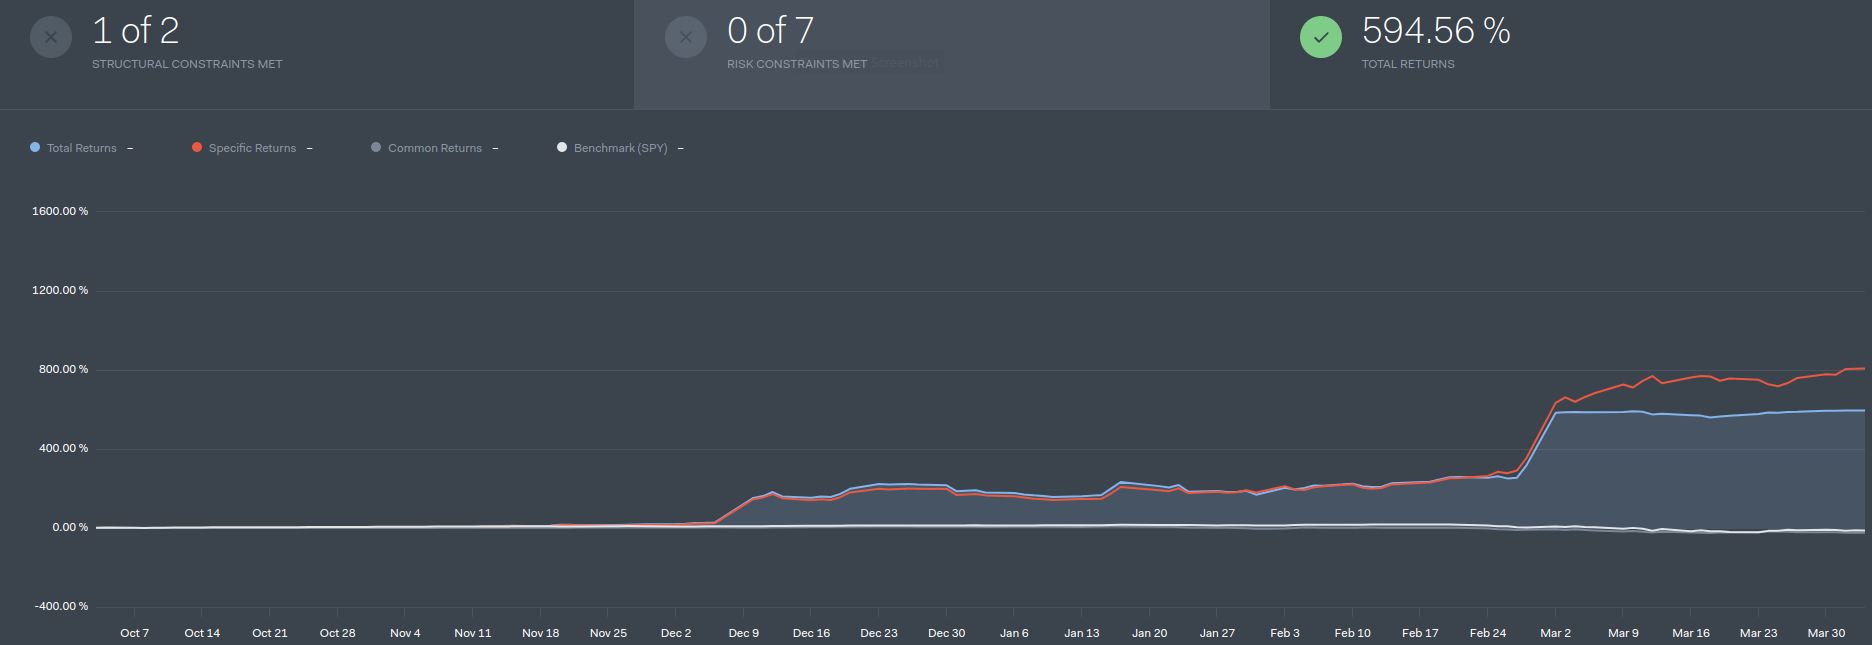
\includegraphics[width=1\linewidth]{inversion_6_meses}
	\caption{Resultados de invertir a 6 meses en el mejor stock posible}
	\label{fig:inversion6meses}
\end{figure}

\begin{figure}
	\centering
	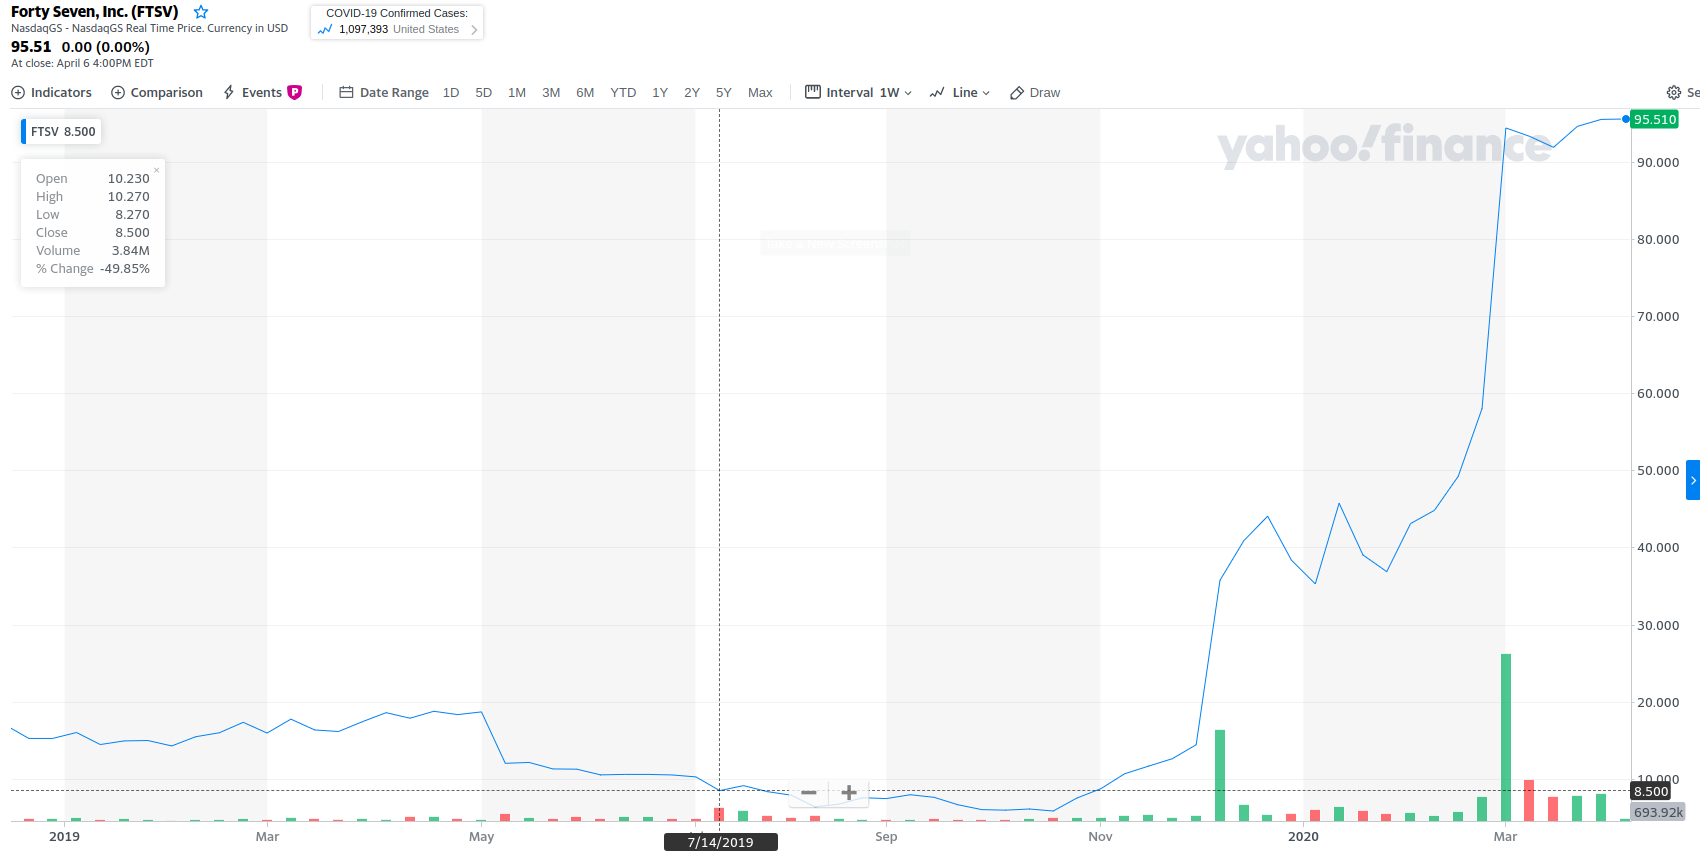
\includegraphics[width=1\linewidth]{yahoo_6_meses}
	\caption{Comportamiento del stock de acuerdo a yahoo finance}
	\label{fig:yahoo6meses}
\end{figure}
\begin{figure}
	\centering
	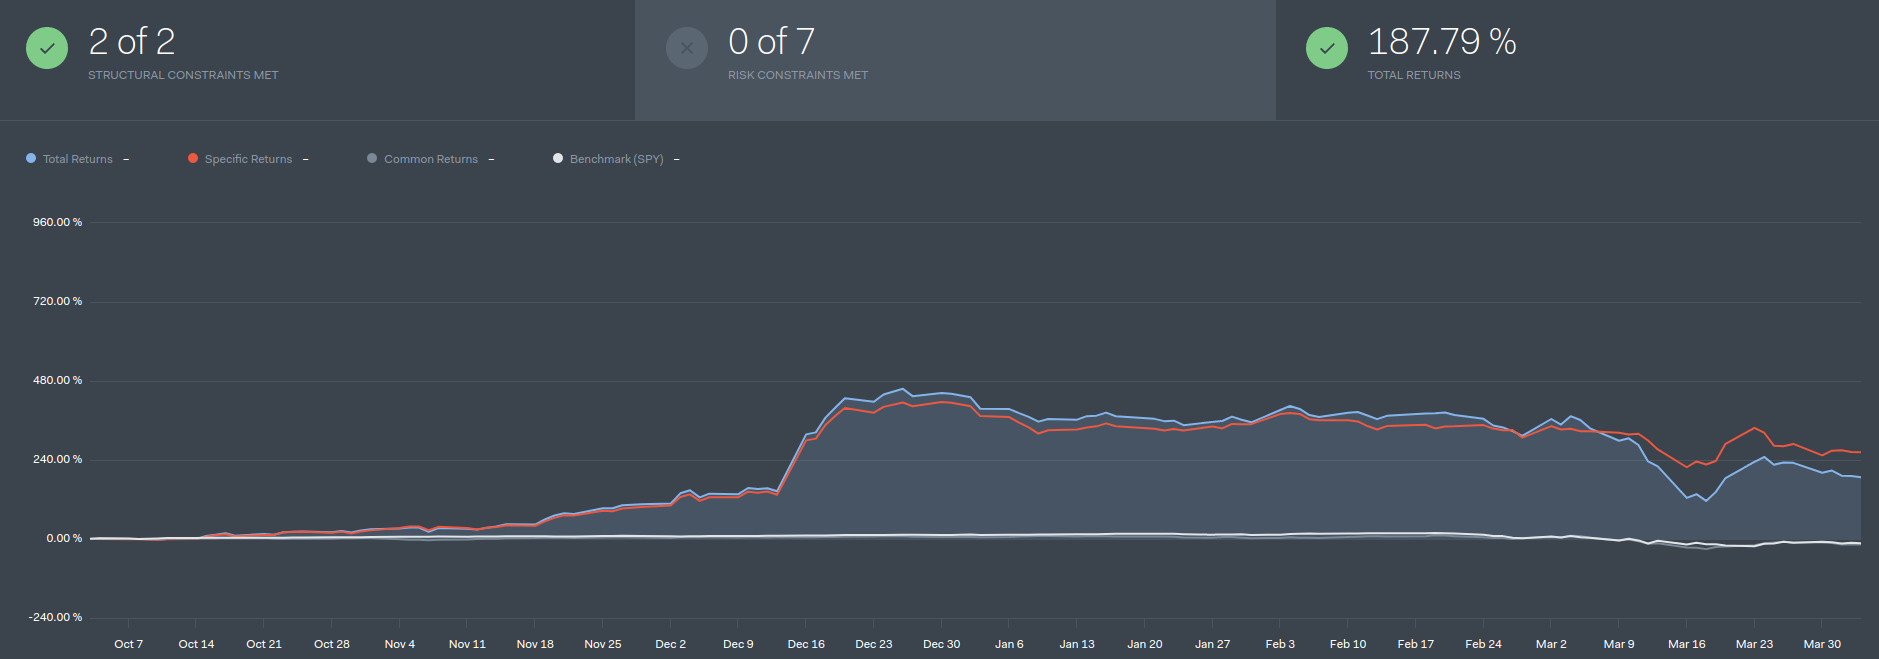
\includegraphics[width=1\linewidth]{inversion_2_anos}
	\caption{}
	\label{fig:inversion2anos}
\end{figure}
\begin{figure}
	\centering
	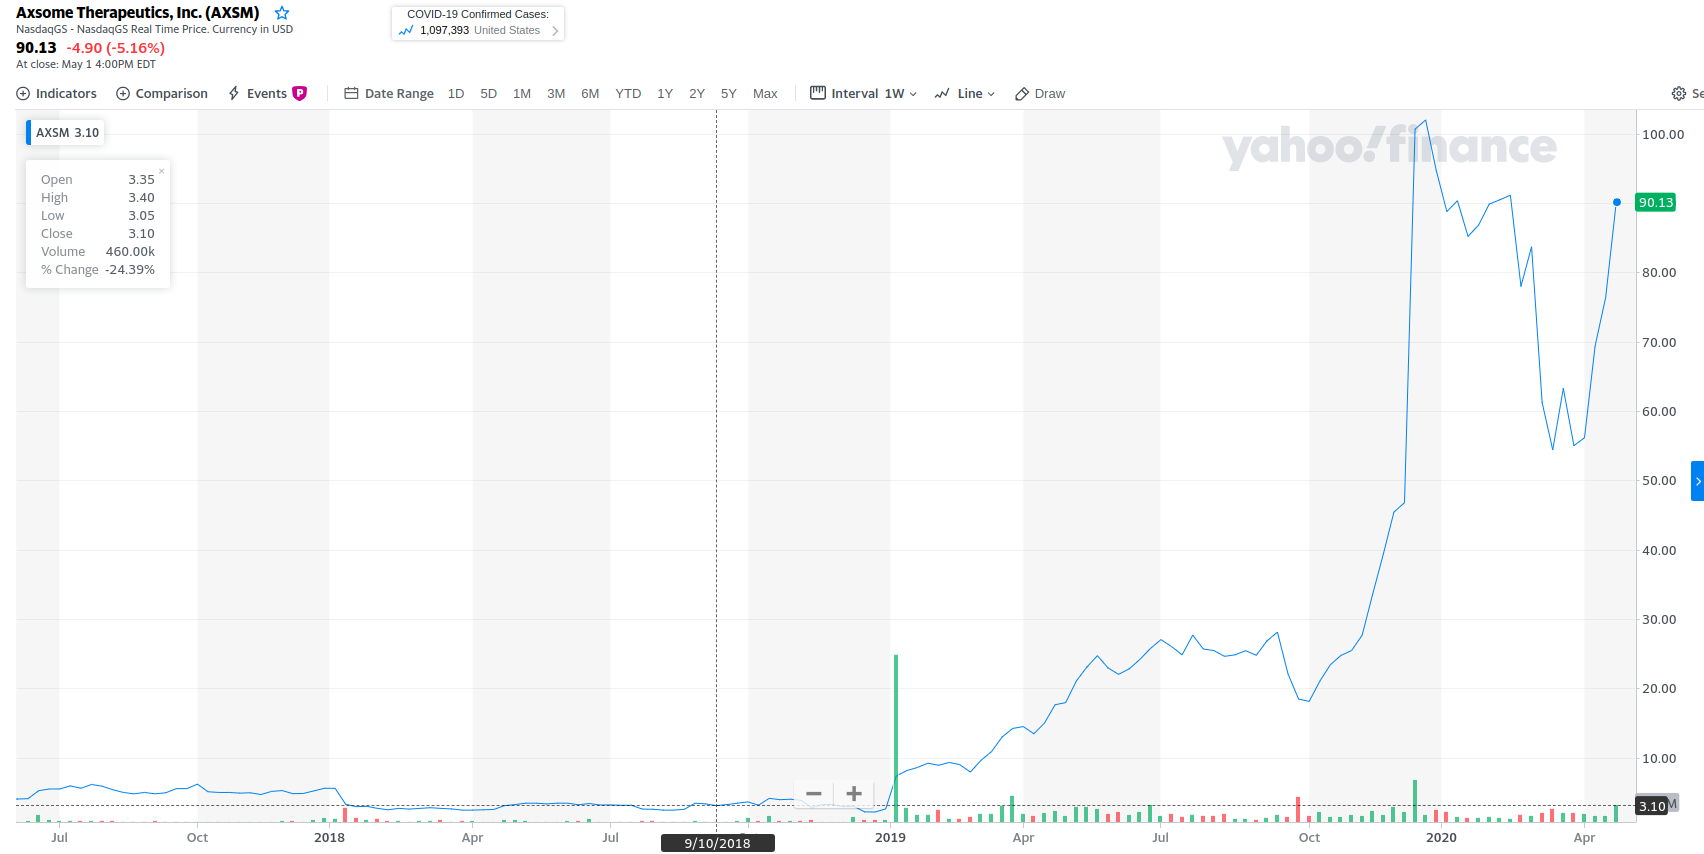
\includegraphics[width=1\linewidth]{yahoo_2_anos}
	\caption{}
	\label{fig:yahoo2anos}
\end{figure}



\end{document}